\documentclass{article}

% if you need to pass options to natbib, use, e.g.:
% \PassOptionsToPackage{numbers, compress}{natbib}
% before loading nips_2016
%
% to avoid loading the natbib package, add option nonatbib:
% \usepackage[nonatbib]{nips_2016}

% \usepackage{nips_2016}

% to compile a camera-ready version, add the [final] option, e.g.:
\usepackage[final]{nips_2016}

\usepackage[utf8]{inputenc} % allow utf-8 input
\usepackage[T1]{fontenc}    % use 8-bit T1 fonts
\usepackage[hidelinks]{hyperref}       % hyperlinks
\usepackage{url}            % simple URL typesetting
\usepackage{booktabs}       % professional-quality tables
\usepackage{amsfonts}       % blackboard math symbols
\usepackage{nicefrac}       % compact symbols for 1/2, etc.
\usepackage{microtype}      % microtypography
\usepackage{amsmath}
\usepackage{enumerate}
\usepackage{graphicx}
\usepackage{placeins}


\newcommand{\figscale}{.7}

\title{Deep Reinforcement Learning in Continuous Multi-agent Environments}

% The \author macro works with any number of authors. There are two
% commands used to separate the names and addresses of multiple
% authors: \And and \AND.
%
% Using \And between authors leaves it to LaTeX to determine where to
% break the lines. Using \AND forces a line break at that point. So,
% if LaTeX puts 3 of 4 authors names on the first line, and the last
% on the second line, try using \AND instead of \And before the third
% author name.

\author{
Ang Li \And%
Michael Kuchnik \And%
Yixin Luo \And%
Rohan Sawhney
}

\begin{document}
% \nipsfinalcopy is no longer used

\maketitle

% % !TEX root=../proposal.tex

\begin{abstract}

\end{abstract}

\begin{figure}[h]
    \centering
    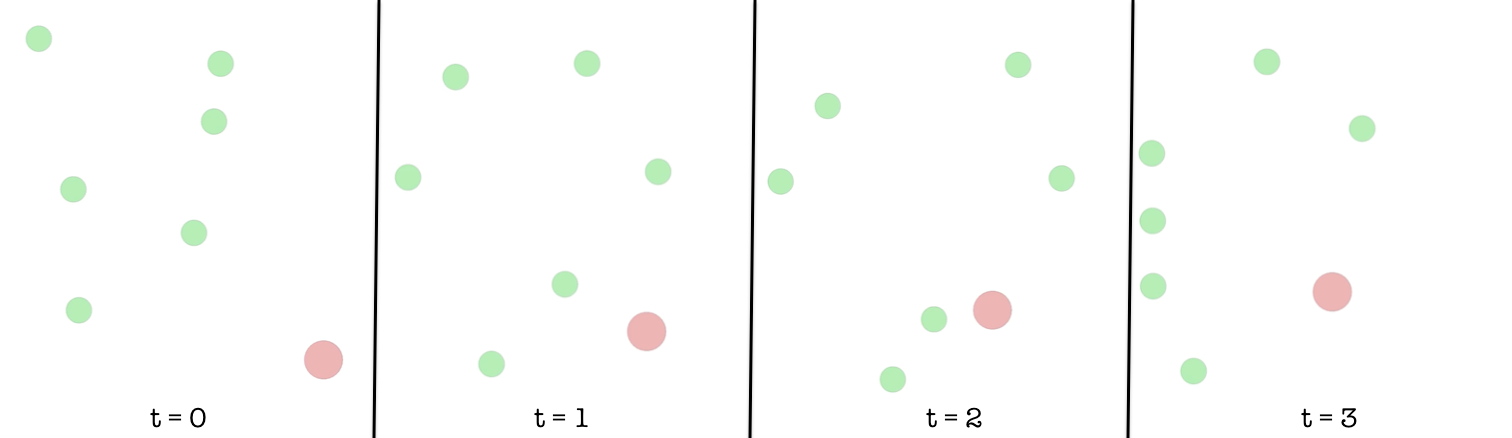
\includegraphics[width=\textwidth]{cover}
	\caption{Illustrations from an episode of Predator Prey with 1 predator (red) and 6 preys (green)}\label{Figure 1}
\end{figure}
% !TEX root=../proposal.tex

\section{Problem Statement}
\label{sec:problem}

Many of the recent successes of deep reinforcement learning have been in
single agent domains, where an agent's reward depends only on its own actions.
However, several important and interesting problems in communication, robotics
and gaming involve interactions between multiple agents. In multi-agent
environments, agents should ideally learn to predict the actions of other
agents while also determining their own actions. Unfortunately, traditional
reinforcement learning approaches such as deep Q-learning and policy gradient
methods struggle to learn in these environments, as they have each agent learn
an independently optimal function.
% TODO we will compare three algorithms (MADDPG, DDPG, and evolutionary)
For our course project, we propose
employing a new algorithm called MADDPG~\cite{lowe2017multi} for centralized
multi-agent learning in various tasks involving cooperation and competition.
Specific examples of tasks where we will use MADDPG include coordinating
traffic signals and communication over a noisy channel. Techniques for
improving the performance of MADDPG will also be explored.

% !TEX root=../report.tex

\section{Background and Related Work}
\label{sec:background}

\subsection{Continuous and High Dimensional Action Spaces}

Many tasks, and in particular those related to physical control, have continuous (real valued) and high dimensional action spaces. A straightforward approach to extending reinforcement learning methods designed for discrete action spaces (e.g. Q learning) to continuous domains is to simply discretize the action space. However, since tasks requiring fine control of actions require a correspondingly finer grained discretization, this leads to an explosion in the number of discrete actions. Large action spaces are difficult to explore efficiently and can make training intractable with traditional methods. In this project, we evaluate the performace of algorithms designed to work with discrete (DQN) as well as continuous actions spaces (DDPG, MADDPG). 

\subsection{Multi-Agent Setting}

Traditional single agent reinforcement learning algorithms typically formulate their environment as a Markov Decision Process (MDP). The multi-agent extension of MDPs with $N$ agents is defined by a set of states $S$ that describe the possible configurations of all agents, a set of actions $A_1, ..., A_N$ and a set of observations $O_1, ..., O_N$. To choose actions, each agent $i$ uses a stochatic policy $\pi_{\theta_i}: O_i \times A_i \rightarrow [0, 1]$ which produces the next state according to the transition function $T: S \times A_1 \times ... \times A_N$. Each agent receives a reward $r_i: S \times A_i \rightarrow \mathbb{R}$ which is a function of the state and the agent's action. Each agent also receives an (potentially partial) observation of the enviorment. The aim of each agent $i$ is to maximize its own total expected return $R_i = \sum_{t=0}^{T} \gamma^{t}r_i^{t}$, where $\gamma$ is the discount factor and $T$ is the reward.

\subsection{Q-Learning and Deep Q Network (DQN)}

Q-Learning is a popular method for reinforcement learning that makes use of an action value function $Q^{\pi}(s, a) = \mathbb{E}[R | s^t = s, a^t = a]$. Many algorithms use the the Bellman equation $Q^{\pi}(s, a) = \mathbb{E}_{s'}[r(s, a) + \gamma \mathbb{E}_{a' \sim \pi}[Q^{\pi}(s', a')]]$ to recursively rewrite and estimate this Q function. A DQN successfully learns the action value function $Q^*$ corresponding to the optimal policy by minimizing the loss:
\begin{equation}
	L(\theta) = \mathbb{E}_{s,a,r,s'\sim D} [(r + \gamma \max_{a'} Q^{*}(s', a') - \bar{Q}^{*}(s, a | \theta))^2]
\end{equation}

where $\bar{Q}$ is the target Q function. Compared to previous Q-Learning techniques, DQN uses deep function approximators in a stable and robust way due to two innovations - 1) the network is trained with a target Q network to give consistent targets during temporal difference backups 2) the network is trained off-policy with samples from a replay buffer $D$ to minimize correlations between samples.

In the multi-agent setting, Q-Learning can be applied by having each agent $i$ learn an independently optimal function $Q_i$. However, there are two fundamental problems in using a DQN in a multi-agent enviroment. First, from any agent's point of view, since the environment is affected by actions taken by other agents unknown to that agent, the state transition function becomes non stationary, violating MDP criteria. Second, and for a similar reason, the experience replay memory becomes inaccurate in approximating the state transitions probabilities.

\subsection{Policy Gradient and Actor Critic Methods}

Another popular choice for single agent reinforcement learning algorithms are the Policy Gradient methods that directly adjust the parameters $\theta$ of the policy in order to maximize the objective $J(\theta) = \mathbb{E}_{s \sim p^{\pi}, a \sim \pi_{\theta}}[R]$ by taking steps in the direction of $\nabla_{\theta} J(\theta)$. There are several advantages of Policy Gradient over value-based techniques, most notably that they are effective in high-dimensional or continuous action spaces, and can learn stochastic policies. The policy gradient theorem gives the following expression
\begin{equation}
	\nabla_{\theta} J(\theta) = \mathbb{E}_{s \sim p^{\pi}, a \sim \pi_{theta}} [\nabla_{\theta} log(\pi_{\theta}(a|s))Q^{\pi}(s, a)]
\end{equation}

for $\nabla_{\theta} J(\theta)$, where $p^\pi$ is the state distribution. Most Policy Gradient methods differ in how they estimate $Q^{\pi}$. For example, REINFORCE is a popular Monte Carlo algorithm that simulates an entire episode to obtain an estimate of the return. Like other single-agent techniques, Policy Gradient methods can also be naively applied to multi-agent reinforcement learning problems. However, since the reward of each agent is highly dependent on other agents’ actions the variance of the gradient updates can be large, making it difficult to train and converge to an optimal policy.

Actor-Critic methods mitigate the high variance problem of Policy Gradient techniques by combining it with value function based techniques. More specifically, Actor-Critic methods learn an approximation of the true action-value function $Q^{\pi} (s, a)$ by e.g., temporal difference learning or deep function approximators. $Q^{\pi} (s, a)$ is called the critic while the actor estimates the policy.

\subsubsection{Deep Deterministic Policy Gradient (DDPG)}
DDPG is an actor critic method that adapts the underyling success of Deep Q-learning to the continuous action domain. DDPG is based on the deterministic  policy gradient algorithm (DPG)~\cite{silver2014deterministic} which rewrites the gradient of the objective $J(\theta)$(Section 2.2) as:
\begin{equation}
	\nabla_{\theta}J(\theta) = \mathbb{E}_{s \sim D} [\nabla_{\theta}\mu_{\theta}(a|s)\nabla_{a} Q^{\mu}(s,a)|_{a = \mu_{\theta}(s)}]
\end{equation}

where $\mu_{\theta}: S \rightarrow A$ are deterministic policies. DDPG approximates both the policy $\mu$ and the critic $Q^{\mu}$ with deep neural networks, sampling trajectories from a replay buffer of experiences and using a target network as in DQN. Note that in the multi-agent setting, each agent is trained individually with DDPG, there is no combined optimization of the agents. However, the MADDPG algorithm, explained in the next section, naturally extends DDPG to the multi-agent setting during training, potentially resulting in much richer behavior between agents.

\subsubsection{Multi Agent Deep Deterministic Policy Gradient (MADDPG)}
MADDPG is a recently developed general-purpose multi-agent learning algorithm that is a simple extension of actor-critic policy gradient methods (specifically DDPG) where the critic is augmented with extra information about the policies of other 
agents while the actor only has access to local information (i.e., its own observations). In this framework of centralized training with decentralized execution, agents don’t need to access the central critic at test time; they learn approximate models of other agents and effectively use them in their own policy learning procedure. Furthermore, since the centralized critic is
learned independently for each agent, this approach can be used to model arbitrary reward structures between agents, including adversarial cases where the rewards are opposing.

More concretely, consider a game with N agents with policies parameterized by $\theta = {\theta_1, ..., \theta_N}$ and let $\mu = {\mu_1, ..., \mu_N}$ be the set of all agent policies. Then, the gradient of the expected return for agent $i$ with deterministic policies $\mu_{\theta_i}$ are given by:
\begin{equation}
\nabla_{\theta_i}J(\mu_i) = E_{x, a \sim D}[\nabla_{\theta_i}\mu_i(a_i|o_i)\nabla_{a_i}Q_i^{\mu}(x, a_1, ..., a_N)|_{a_i = \mu_i(o_i)}]
\end{equation}

Here the experience replay buffer $D$ contains the tuples $(x, x_0, a_1,..., a_N, r_1,..., r_N)$, recording experiences of all agents. $Q^{\mu}_i$ is the centralized action-value function that takes as input the actions of all agents, in addition to some state information x, and outputs the Q-value for agent i. Since each $Q^{\mu}_i$ is learned separately, agents can have 
arbitrary reward structures, including conflicting rewards in a competitive setting.  

A primary motivation behind MADDPG is that, if the actions taken by all the agents are known, then the environment is stationary as the policies change. This is not the case if the actions of other agents are not explicity conditioned on, as done for most traditional reinforcement learning. Finally, note that the policies of other agents needs to be known to compute the loss. Knowing the observations and policies of other agents is not a particularly restrictive assumption; if the goal is to train agents to exhibit complex communicative behaviour in simulation, this information is often available to all agents. However, MADDPG also allows for this assumption to be relaxed by learning the policies of other agents from observations.


% !TEX root=../report.tex

\section{Environment and Applications}
\label{sec:application}

In this project, we use the OpenAI Gym framework~\cite{gym.openai16}, which
generates virtually infinite amount of data for training and testing our
neural network. This framework includes various gym environments that simulate
various reinforcement learning settings. Each gym environment defines the
\emph{state space} (i.e., all possible states of the environment) and the
action space (i.e., all possible actions of the agent). Note that a gym
environment is turn-based, i.e., the agent can only take one action per time
step to influence the state at the next time step. In each time step, the
environment computes the next state and the immediate reward for each agent,
and decide if the episode is finished or not. These pieces of information
(i.e., the immediate reward and the episode finished signal) are used by each
agent to decide the best action in the next step. We refer the readers to
Section~\ref{sec:background:problem} for a detailed explanation of a classical
reinforcement learning problem setting.

\subsection{The Predator-Pray Environment}

We develop a modified version of the \emph{``predator-pray''} scenario
in the ``multi-agent particle'' environment suite developed by prior
work~\cite{lowe2017multi, mordatch2017emergence}, and train our
neural-network-based agents. In the original classic predator-prey game, $N$
slower \emph{cooperating agents} must chase the faster \emph{adversary}
around a randomly
generated environment with $L$ large landmarks impeding the way. Each time the
cooperative agents collide with an adversary, the agents are rewarded
while the adversary is penalized. Agents observe the relative positions and
velocities of the adversary, and the positions of the landmarks. We introduce
the state space, action space, the reward function, and our modifications to
the scenario.

\paragraph{State Space.} In the predator-pray scenario, each agent can only
observe its own state (i.e., $state[i]$). At each step, the environment
returns these states concatenated into a list, which is then distributed to
each individual agent accordingly. The $state[i]$ of each agent contains 
(1)~the velocity and the location of itself in the x- and y-coordinate,
(2)~the relative x- and y-coordinate of two landmarks,
(3)~the relative x- and y-coordinate of all other agents, and
(4)~the x- and y-directional velocity of of the escaping adversary.

\paragraph{Action Space.} At each step, each agent can take an action (i.e.,
$action[i]$) to move itself. Similar to the sate, all agents' actions are
concatenated into a list and send to the environment. The $action[i]$ of each
agent contains a no-action signal, and the movements towards four directions 
(i.e., right, left, down, or up). In the discrete action space used for DQN,
the action is simply an one-hot encoding of the five possible actions, where
each action has a fixed amplitude. In continuous action space used for DDPG
and MADDPG, the environment computes the amplitude of movement along the
x-axis (i.e., $right - left$) and the y-axis (i.e., $up - down$).

\paragraph{Reward Function.} In the original environment, all agents receive
a fixed positive reward if any agent has collided into the adversary. If such
collision happens, the same amount of negative reward is taken out of the
adversary. In order to keep the game visible on the screen and to reduce the
state space, the adversary also receives negative reward when it goes out of
the computer screen.

\paragraph{Our Modifications.} First, we modify the reward function to make
the scenario more interesting. In addition to the reward function in the
original version, we added positive reward to the adversary for how far it
is to the agents, measured in l2 distance. Similarly, a negative reward is add
to the agent for how far it is to the adversary.
Second, we modify the original predator-pray
scenario to test different number of agents and adversaries. We included
results for (1)~1 agent vs. 1 adversary, (2)~1 agent vs. 2 adversaries, and 
(3)~2 agents vs. 1 adversary. Third, we made the scenario into an episodic
game. The episode never ends in the original version. The episode now ends
when any agent or adversary goes out of the screen.


% !TEX root=../report.tex

\section{Experiments}
\label{sec:experiment}


\subsection{DQN}
\label{sec:experiment:dqn}


\subsubsection{One Agents vs. One Adversary Results}
\label{sec:experiment:dqn:1vs1}


\begin{figure}[h]
  \centering
  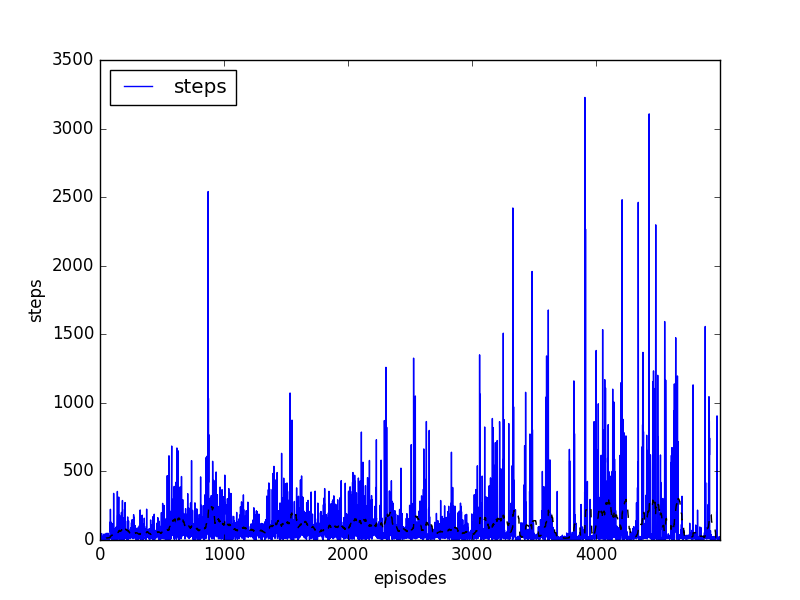
\includegraphics[trim=10 10 10 10,clip,width=\figscale\linewidth]
  {../results/dqn_1vs1/steps.png}
  \caption{Number of steps per episode over training episode for DQN.}
  \label{fig:dqn-1vs1}
\end{figure}
\FloatBarrier


\begin{figure}[h]
  \centering
  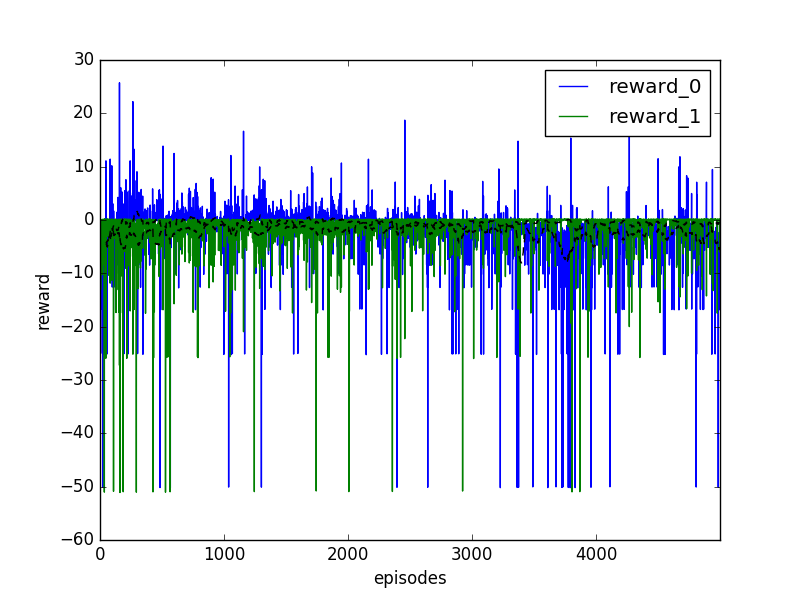
\includegraphics[trim=10 10 10 10,clip,width=\figscale\linewidth]
  {../results/dqn_1vs1/reward.png}
  \caption{Cumulative reward per episode over training episode for DQN.}
  \label{fig:dqn-1vs1}
\end{figure}
\FloatBarrier


\begin{figure}[h]
  \centering
  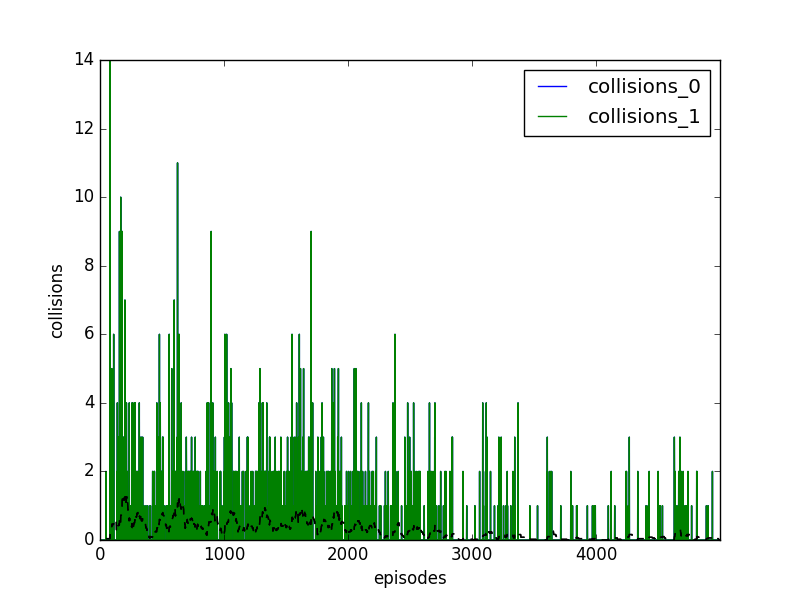
\includegraphics[trim=10 10 10 10,clip,width=\figscale\linewidth]
  {../results/dqn_1vs1/collisions.png}
  \caption{Number of collisions per episode over training episode for DQN.}
  \label{fig:dqn-1vs1}
\end{figure}
\FloatBarrier


\begin{figure}[h]
  \centering
  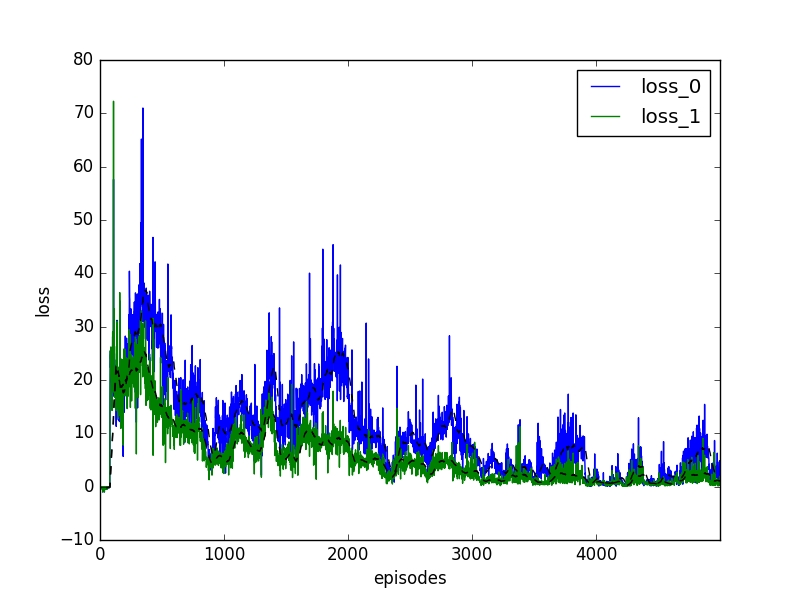
\includegraphics[trim=10 10 10 10,clip,width=\figscale\linewidth]
  {../results/dqn_1vs1/loss.png}
  \caption{Average loss per episode over training episode for DQN.}
  \label{fig:dqn-1vs1}
\end{figure}
\FloatBarrier


\subsubsection{Two Agents vs. One Adversary Results}
\label{sec:experiment:dqn:1vs2}


\begin{figure}[h]
  \centering
  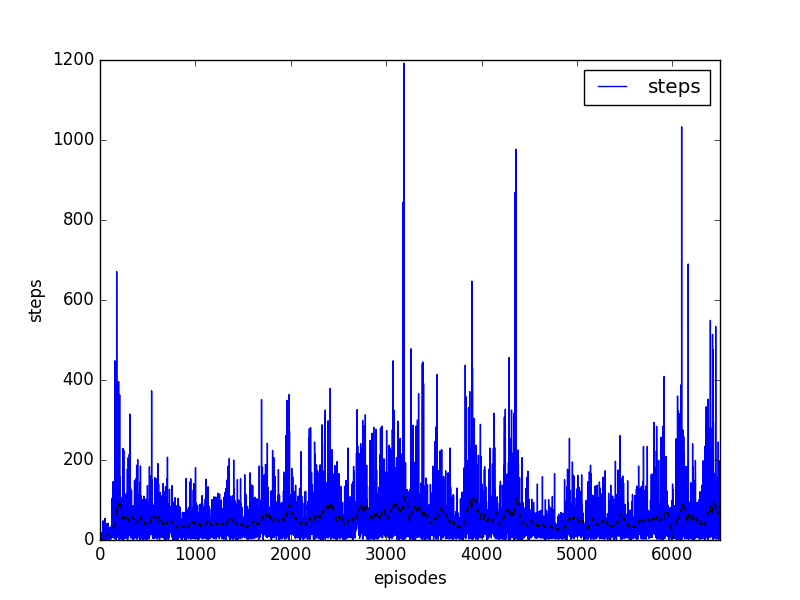
\includegraphics[trim=10 10 10 10,clip,width=\figscale\linewidth]
  {../results/dqn_1vs2/steps.png}
  \caption{Number of steps per episode over training episode for DQN.}
  \label{fig:dqn-1vs2}
\end{figure}
\FloatBarrier


\begin{figure}[h]
  \centering
  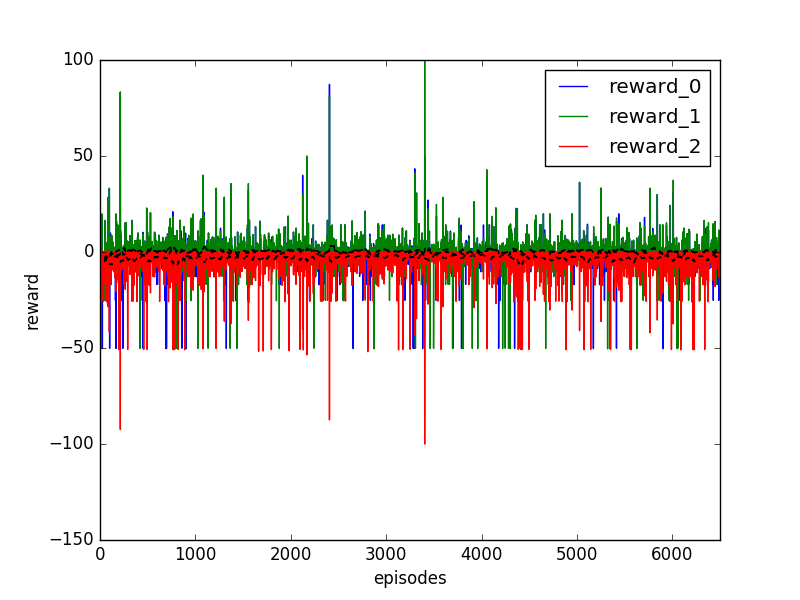
\includegraphics[trim=10 10 10 10,clip,width=\figscale\linewidth]
  {../results/dqn_1vs2/reward.png}
  \caption{Cumulative reward per episode over training episode for DQN.}
  \label{fig:dqn-1vs2}
\end{figure}
\FloatBarrier


\begin{figure}[h]
  \centering
  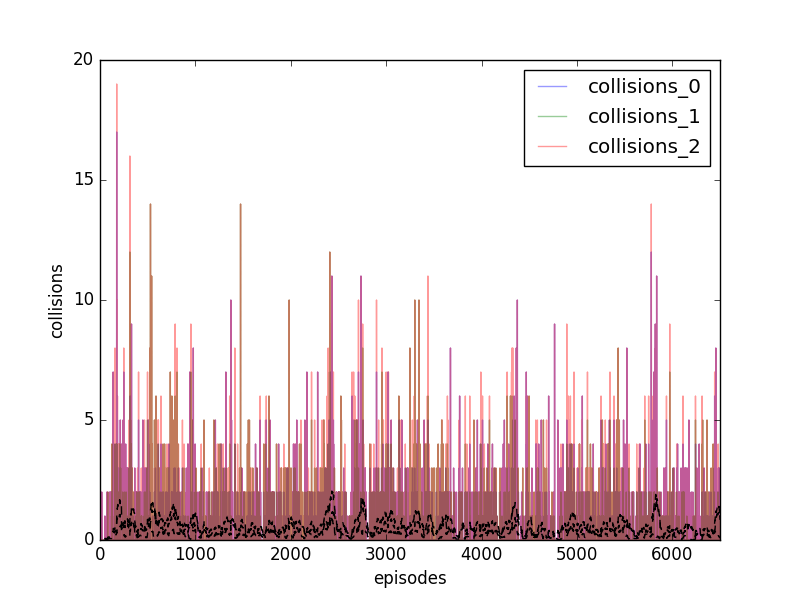
\includegraphics[trim=10 10 10 10,clip,width=\figscale\linewidth]
  {../results/dqn_1vs2/collisions.png}
  \caption{Number of collisions per episode over training episode for DQN.}
  \label{fig:dqn-1vs2}
\end{figure}
\FloatBarrier


\begin{figure}[h]
  \centering
  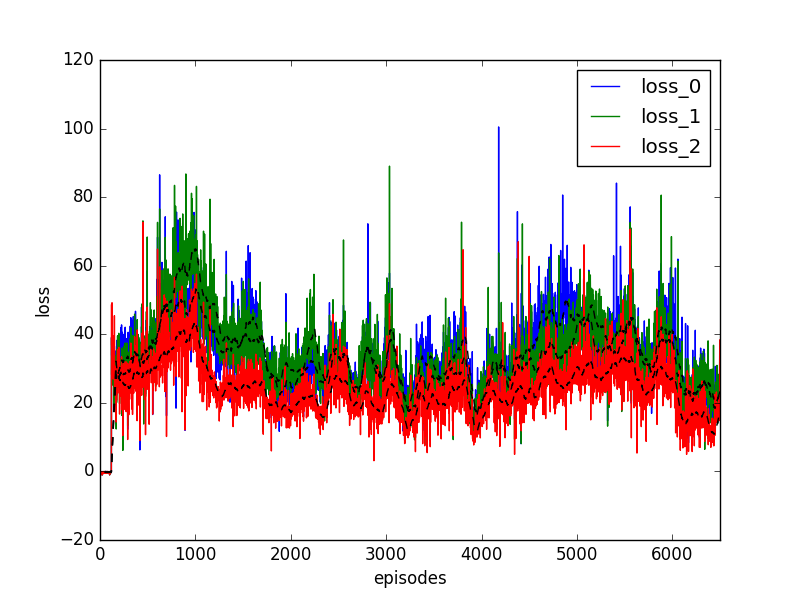
\includegraphics[trim=10 10 10 10,clip,width=\figscale\linewidth]
  {../results/dqn_1vs2/loss.png}
  \caption{Average loss per episode over training episode for DQN.}
  \label{fig:dqn-1vs2}
\end{figure}
\FloatBarrier


\subsubsection{One Agents vs. Two Adversary Results}
\label{sec:experiment:dqn:2vs1}


\begin{figure}[h]
  \centering
  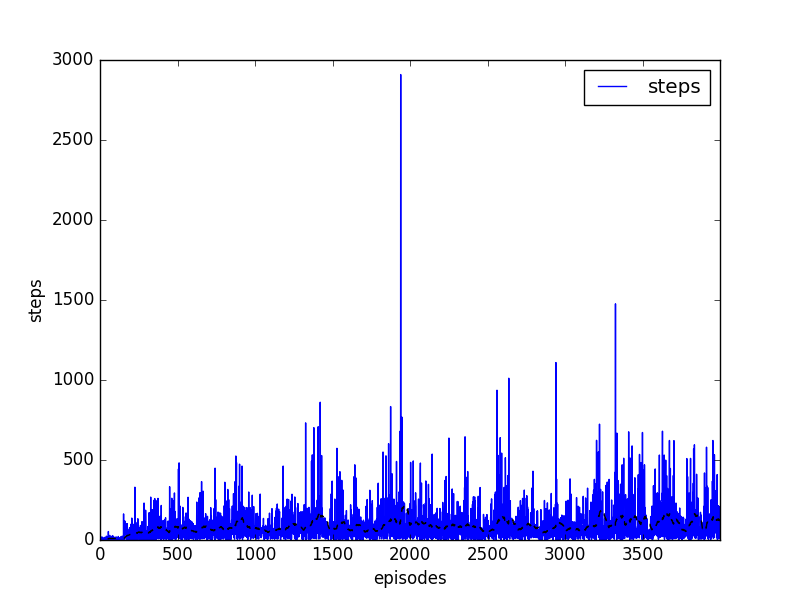
\includegraphics[trim=10 10 10 10,clip,width=\figscale\linewidth]
  {../results/dqn_2vs1/steps.png}
  \caption{Number of steps per episode over training episode for DQN.}
  \label{fig:dqn-2vs1}
\end{figure}
\FloatBarrier


\begin{figure}[h]
  \centering
  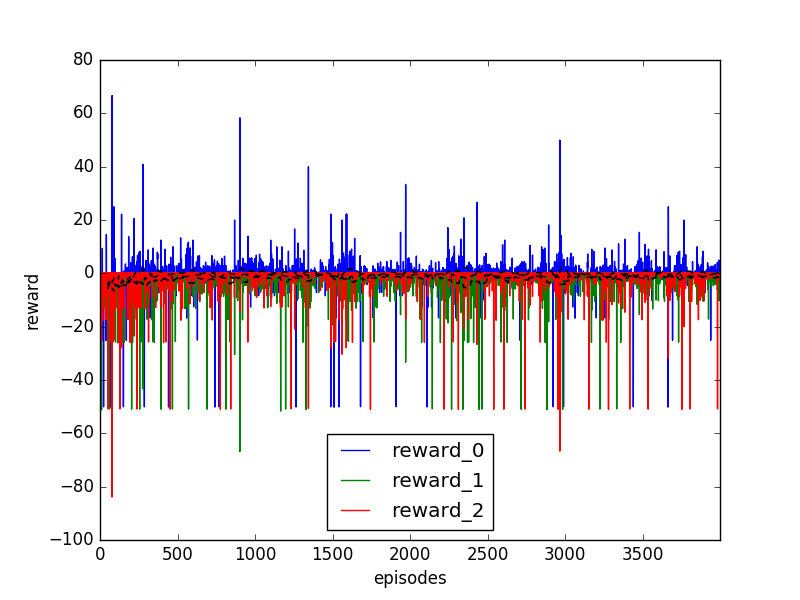
\includegraphics[trim=10 10 10 10,clip,width=\figscale\linewidth]
  {../results/dqn_2vs1/reward.png}
  \caption{Cumulative reward per episode over training episode for DQN.}
  \label{fig:dqn-2vs1}
\end{figure}
\FloatBarrier


\begin{figure}[h]
  \centering
  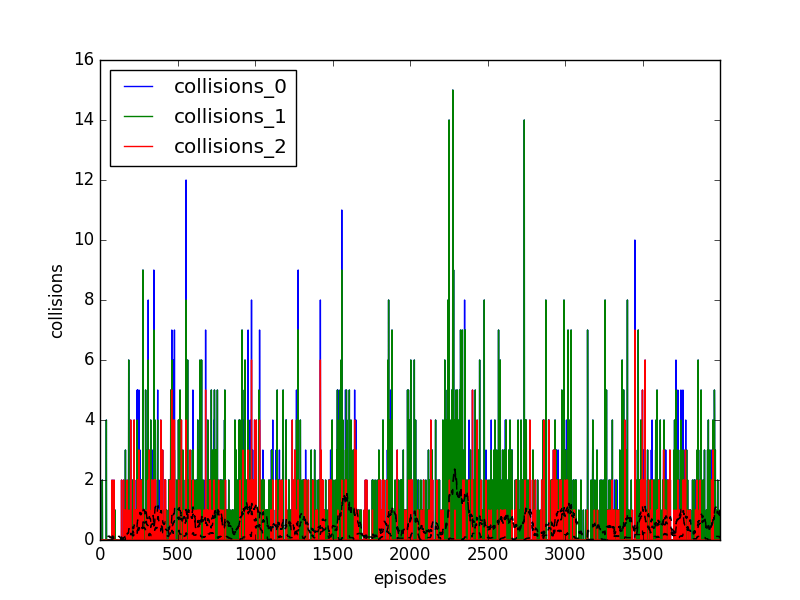
\includegraphics[trim=10 10 10 10,clip,width=\figscale\linewidth]
  {../results/dqn_2vs1/collisions.png}
  \caption{Number of collisions per episode over training episode for DQN.}
  \label{fig:dqn-2vs1}
\end{figure}
\FloatBarrier


\begin{figure}[h]
  \centering
  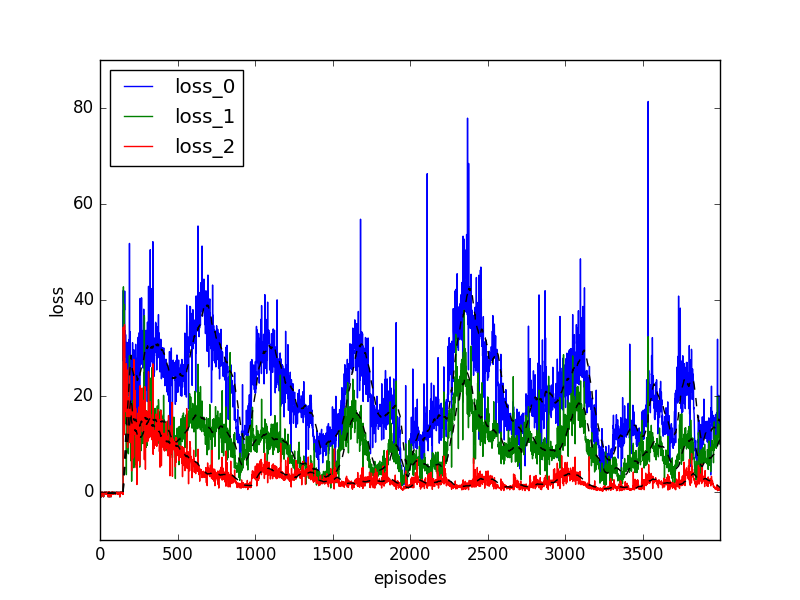
\includegraphics[trim=10 10 10 10,clip,width=\figscale\linewidth]
  {../results/dqn_2vs1/loss.png}
  \caption{Average loss per episode over training episode for DQN.}
  \label{fig:dqn-2vs1}
\end{figure}
\FloatBarrier


\subsection{DDPG}
\label{sec:experiment:ddpg}


\subsubsection{One Agents vs. One Adversary Results}
\label{sec:experiment:ddpg:1vs1}


\begin{figure}[h]
  \centering
  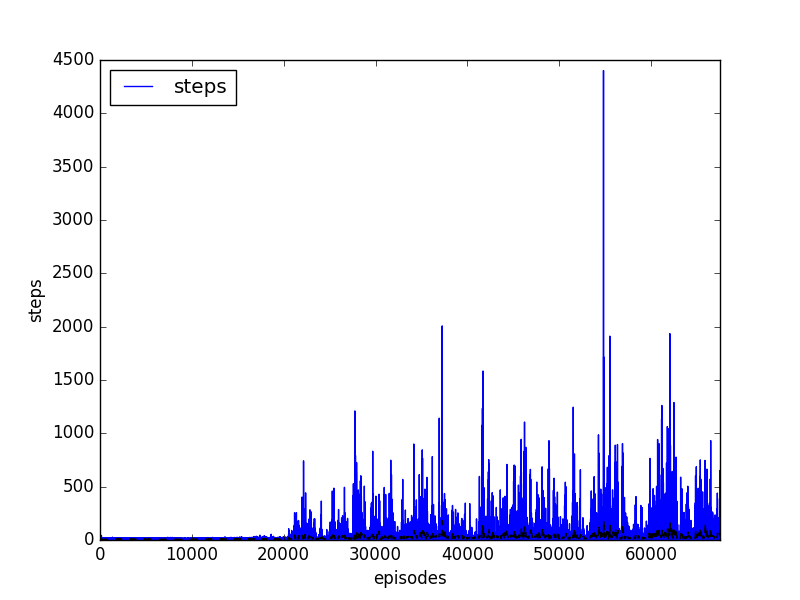
\includegraphics[trim=10 10 10 10,clip,width=\figscale\linewidth]
  {../results/ddpg_1vs1/steps.png}
  \caption{Number of steps per episode over training episode for DDPG.}
  \label{fig:ddpg-1vs1}
\end{figure}
\FloatBarrier


\begin{figure}[h]
  \centering
  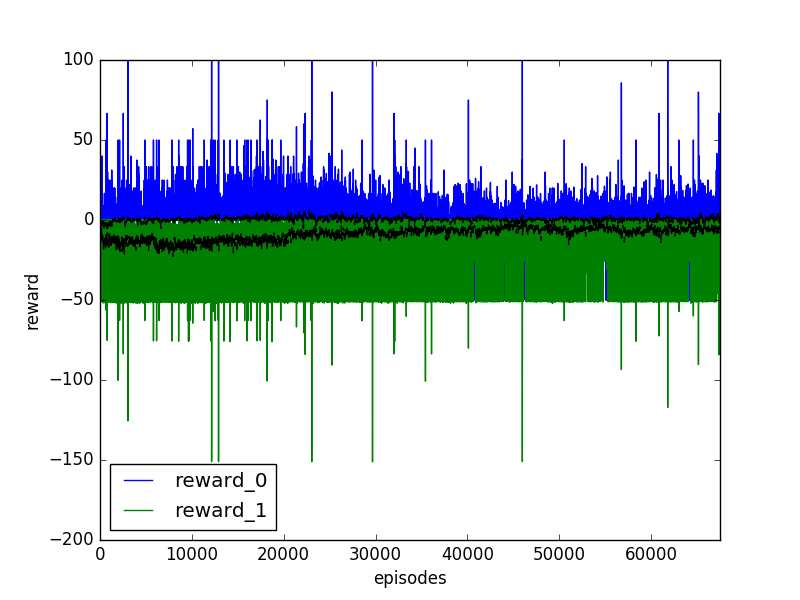
\includegraphics[trim=10 10 10 10,clip,width=\figscale\linewidth]
  {../results/ddpg_1vs1/reward.png}
  \caption{Cumulative reward per episode over training episode for DDPG.}
  \label{fig:ddpg-1vs1}
\end{figure}
\FloatBarrier


\begin{figure}[h]
  \centering
  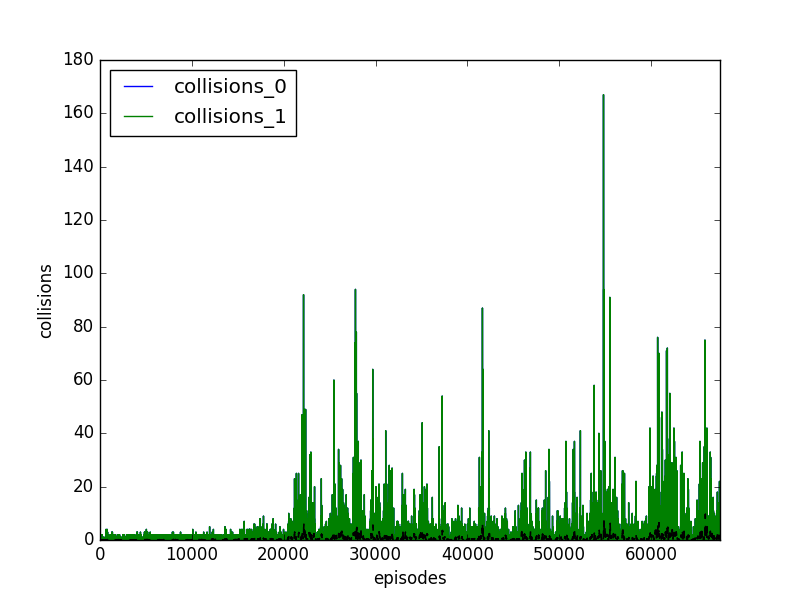
\includegraphics[trim=10 10 10 10,clip,width=\figscale\linewidth]
  {../results/ddpg_1vs1/collisions.png}
  \caption{Number of collisions per episode over training episode for DDPG.}
  \label{fig:ddpg-1vs1}
\end{figure}
\FloatBarrier


\begin{figure}[h]
  \centering
  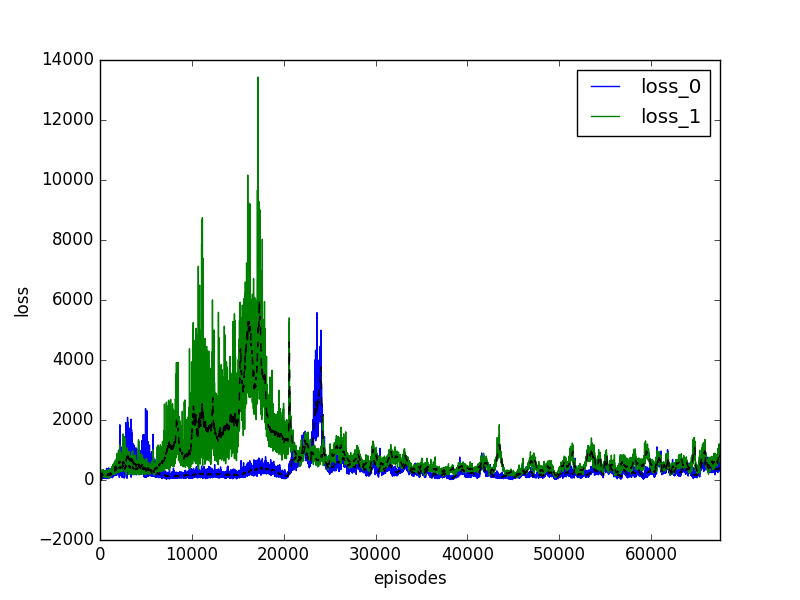
\includegraphics[trim=10 10 10 10,clip,width=\figscale\linewidth]
  {../results/ddpg_1vs1/loss.png}
  \caption{Average loss per episode over training episode for DDPG.}
  \label{fig:ddpg-1vs1}
\end{figure}
\FloatBarrier


\subsubsection{Two Agents vs. One Adversary Results}
\label{sec:experiment:ddpg:1vs2}


\begin{figure}[h]
  \centering
  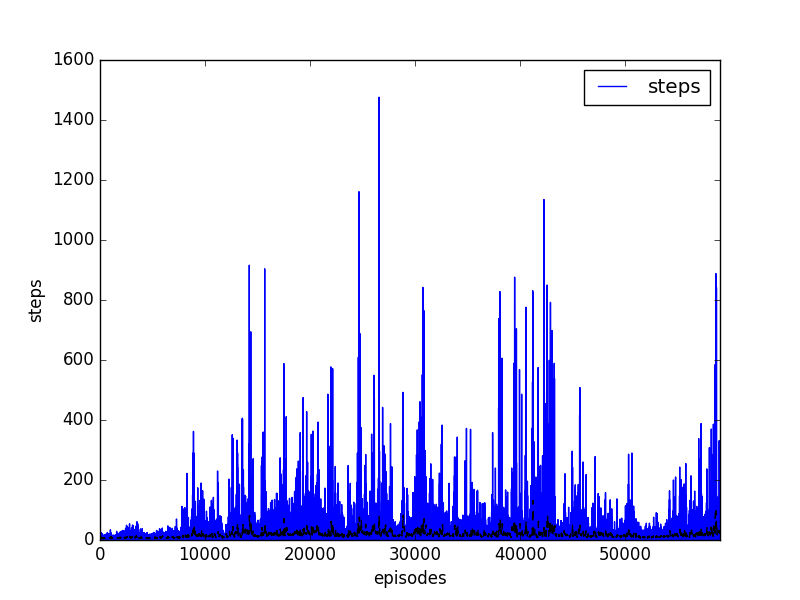
\includegraphics[trim=10 10 10 10,clip,width=\figscale\linewidth]
  {../results/ddpg_1vs2/steps.png}
  \caption{Number of steps per episode over training episode for DDPG.}
  \label{fig:ddpg-1vs2}
\end{figure}
\FloatBarrier


\begin{figure}[h]
  \centering
  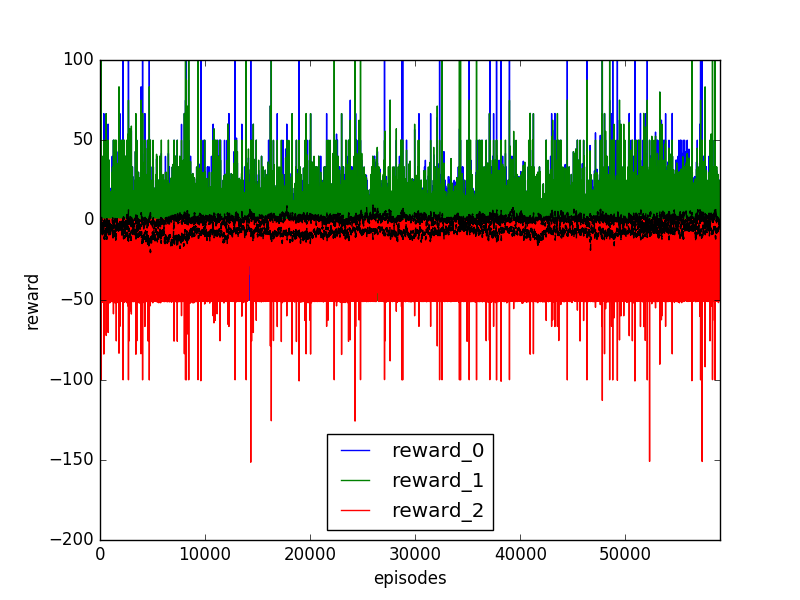
\includegraphics[trim=10 10 10 10,clip,width=\figscale\linewidth]
  {../results/ddpg_1vs2/reward.png}
  \caption{Cumulative reward per episode over training episode for DDPG.}
  \label{fig:ddpg-1vs2}
\end{figure}
\FloatBarrier


\begin{figure}[h]
  \centering
  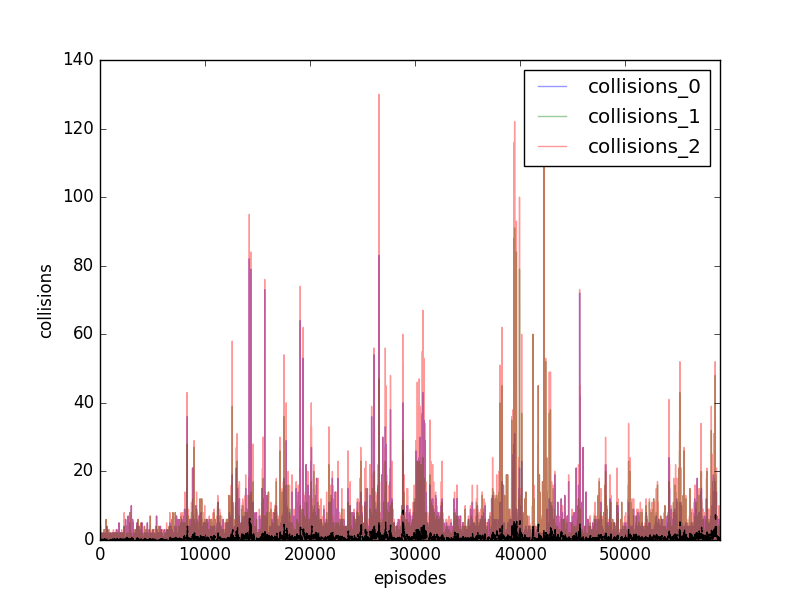
\includegraphics[trim=10 10 10 10,clip,width=\figscale\linewidth]
  {../results/ddpg_1vs2/collisions.png}
  \caption{Number of collisions per episode over training episode for DDPG.}
  \label{fig:ddpg-1vs2}
\end{figure}
\FloatBarrier


\begin{figure}[h]
  \centering
  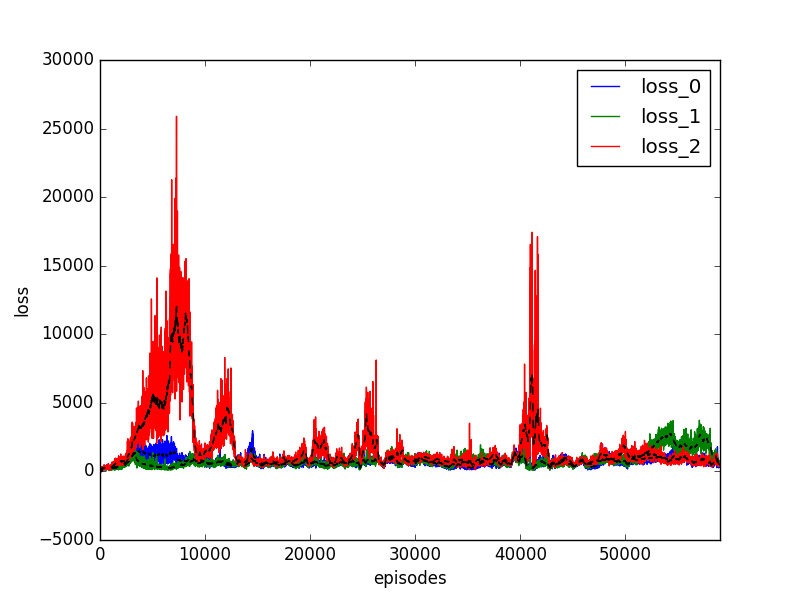
\includegraphics[trim=10 10 10 10,clip,width=\figscale\linewidth]
  {../results/ddpg_1vs2/loss.png}
  \caption{Average loss per episode over training episode for DDPG.}
  \label{fig:ddpg-1vs2}
\end{figure}
\FloatBarrier


\subsubsection{One Agents vs. Two Adversary Results}
\label{sec:experiment:ddpg:2vs1}


\begin{figure}[h]
  \centering
  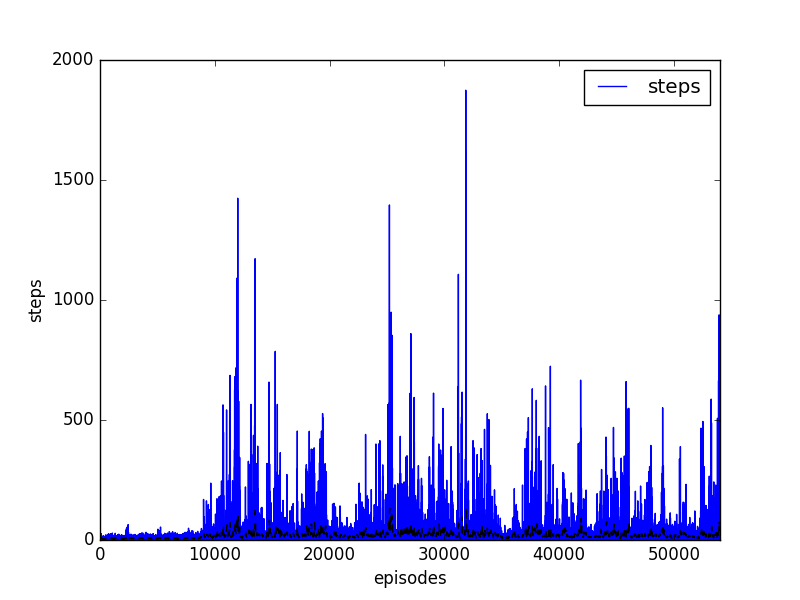
\includegraphics[trim=10 10 10 10,clip,width=\figscale\linewidth]
  {../results/ddpg_2vs1/steps.png}
  \caption{Number of steps per episode over training episode for DDPG.}
  \label{fig:ddpg-2vs1}
\end{figure}
\FloatBarrier


\begin{figure}[h]
  \centering
  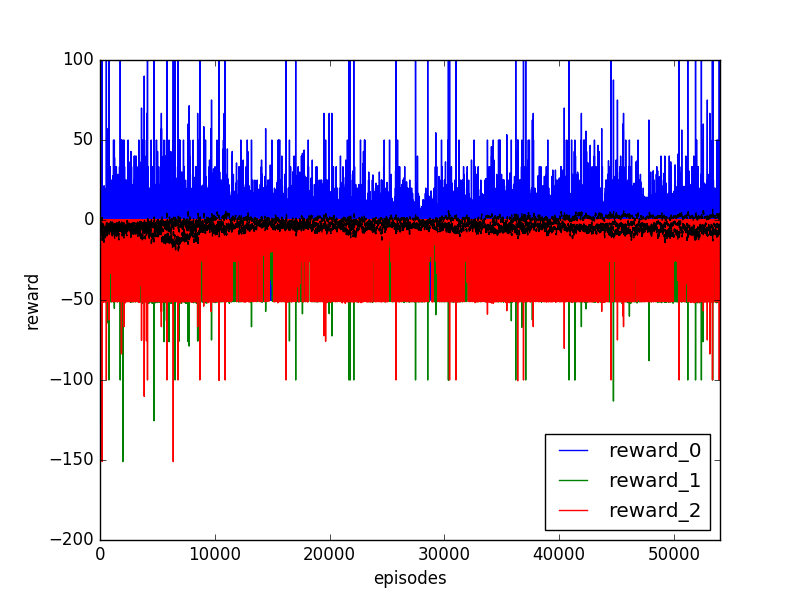
\includegraphics[trim=10 10 10 10,clip,width=\figscale\linewidth]
  {../results/ddpg_2vs1/reward.png}
  \caption{Cumulative reward per episode over training episode for DDPG.}
  \label{fig:ddpg-2vs1}
\end{figure}
\FloatBarrier


\begin{figure}[h]
  \centering
  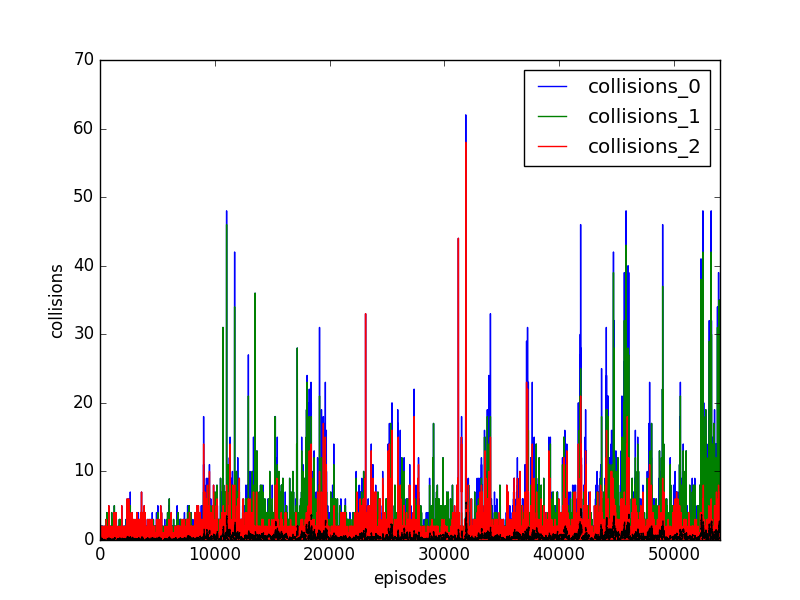
\includegraphics[trim=10 10 10 10,clip,width=\figscale\linewidth]
  {../results/ddpg_2vs1/collisions.png}
  \caption{Number of collisions per episode over training episode for DDPG.}
  \label{fig:ddpg-2vs1}
\end{figure}
\FloatBarrier


\begin{figure}[h]
  \centering
  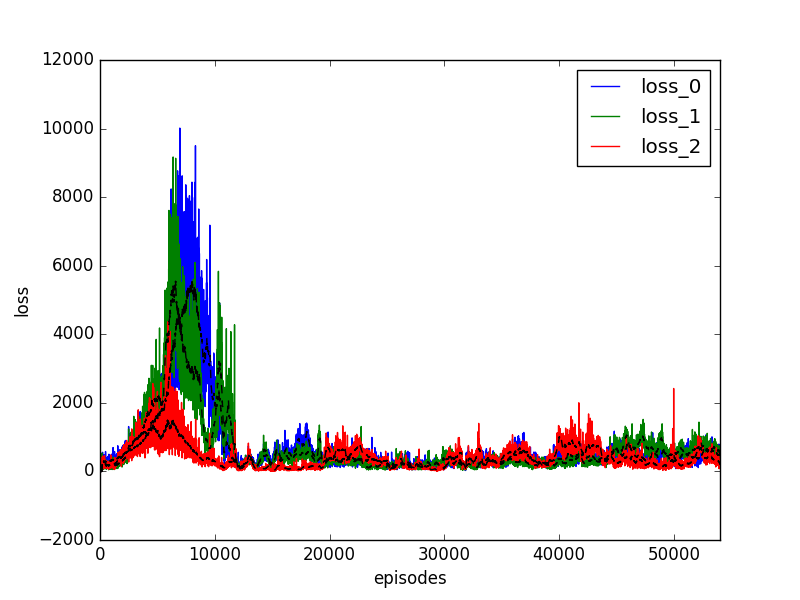
\includegraphics[trim=10 10 10 10,clip,width=\figscale\linewidth]
  {../results/ddpg_2vs1/loss.png}
  \caption{Average loss per episode over training episode for DDPG.}
  \label{fig:ddpg-2vs1}
\end{figure}
\FloatBarrier


\subsection{MADDPG}
\label{sec:experiment:maddpg}


\subsubsection{One Agents vs. One Adversary Results}
\label{sec:experiment:maddpg:1vs1}


\begin{figure}[h]
  \centering
  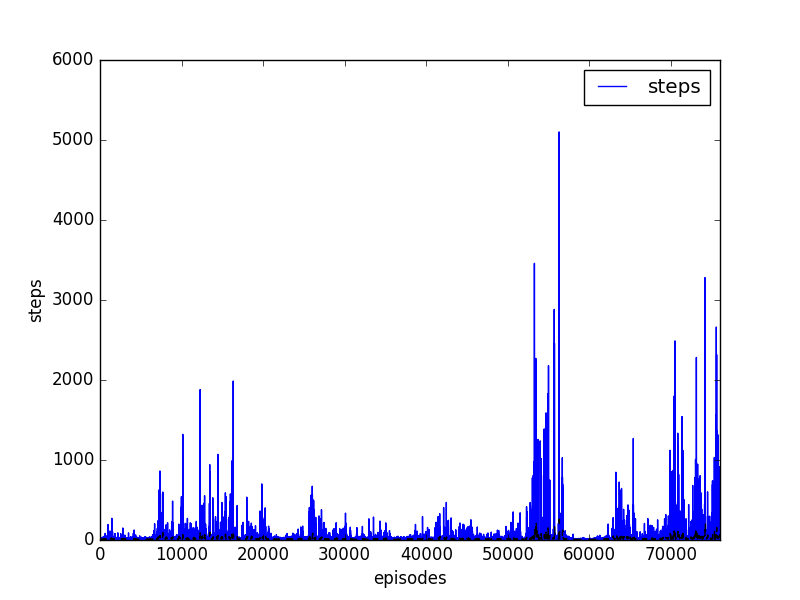
\includegraphics[trim=10 10 10 10,clip,width=\figscale\linewidth]
  {../results/maddpg_1vs1/steps.png}
  \caption{Number of steps per episode over training episode for MADDPG.}
  \label{fig:maddpg-1vs1}
\end{figure}
\FloatBarrier


\begin{figure}[h]
  \centering
  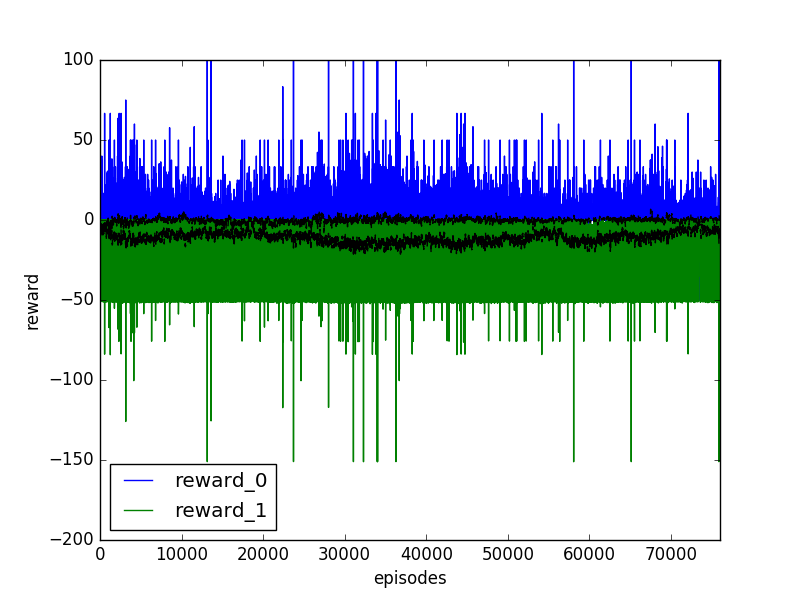
\includegraphics[trim=10 10 10 10,clip,width=\figscale\linewidth]
  {../results/maddpg_1vs1/reward.png}
  \caption{Cumulative reward per episode over training episode for MADDPG.}
  \label{fig:maddpg-1vs1}
\end{figure}
\FloatBarrier


\begin{figure}[h]
  \centering
  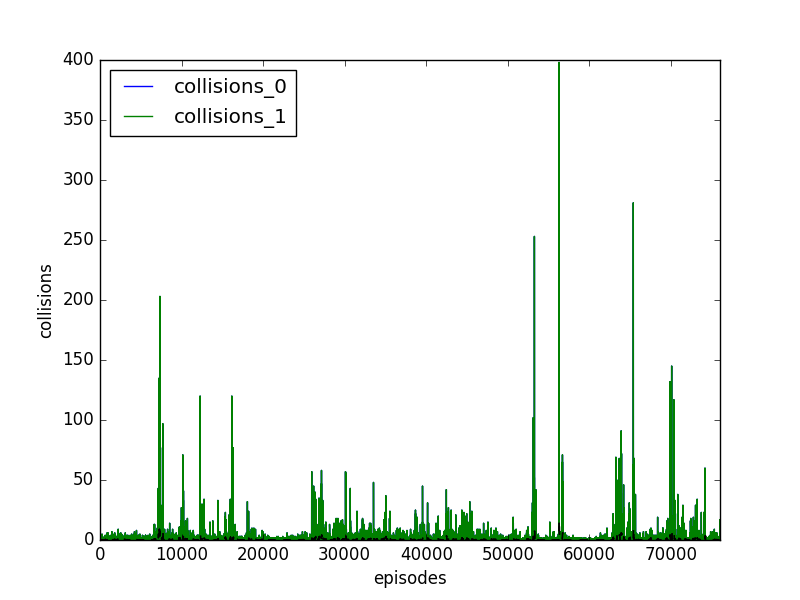
\includegraphics[trim=10 10 10 10,clip,width=\figscale\linewidth]
  {../results/maddpg_1vs1/collisions.png}
  \caption{Number of collisions per episode over training episode for MADDPG.}
  \label{fig:maddpg-1vs1}
\end{figure}
\FloatBarrier


\begin{figure}[h]
  \centering
  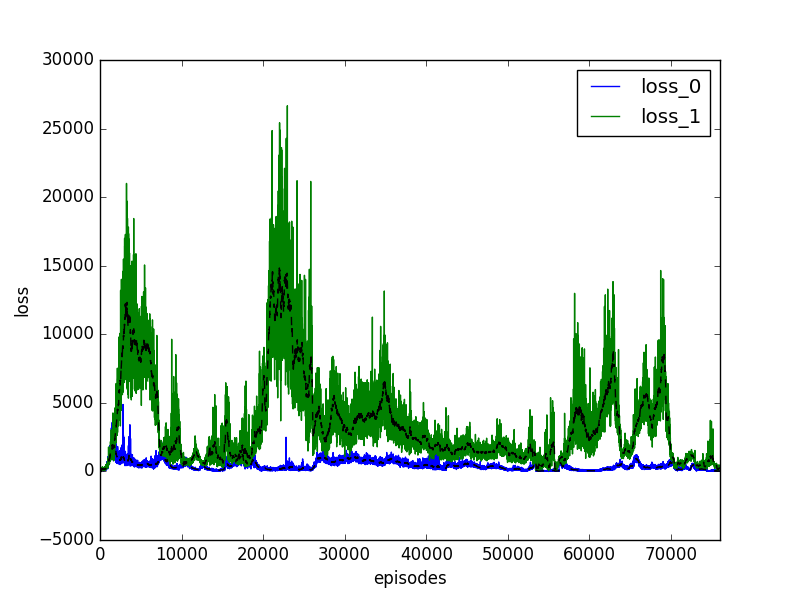
\includegraphics[trim=10 10 10 10,clip,width=\figscale\linewidth]
  {../results/maddpg_1vs1/loss.png}
  \caption{Average loss per episode over training episode for MADDPG.}
  \label{fig:maddpg-1vs1}
\end{figure}
\FloatBarrier


\subsubsection{Two Agents vs. One Adversary Results}
\label{sec:experiment:maddpg:1vs2}


\begin{figure}[h]
  \centering
  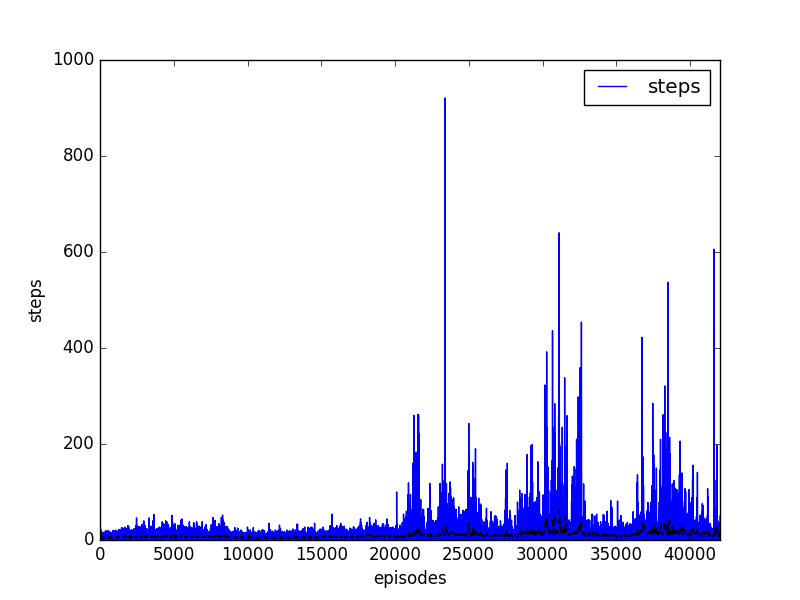
\includegraphics[trim=10 10 10 10,clip,width=\figscale\linewidth]
  {../results/maddpg_1vs2/steps.png}
  \caption{Number of steps per episode over training episode for MADDPG.}
  \label{fig:maddpg-1vs2}
\end{figure}
\FloatBarrier


\begin{figure}[h]
  \centering
  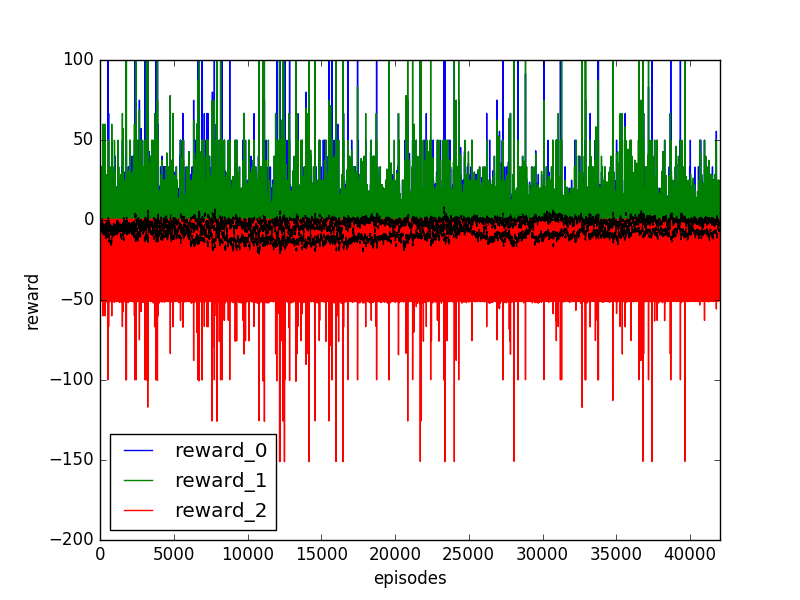
\includegraphics[trim=10 10 10 10,clip,width=\figscale\linewidth]
  {../results/maddpg_1vs2/reward.png}
  \caption{Cumulative reward per episode over training episode for MADDPG.}
  \label{fig:maddpg-1vs2}
\end{figure}
\FloatBarrier


\begin{figure}[h]
  \centering
  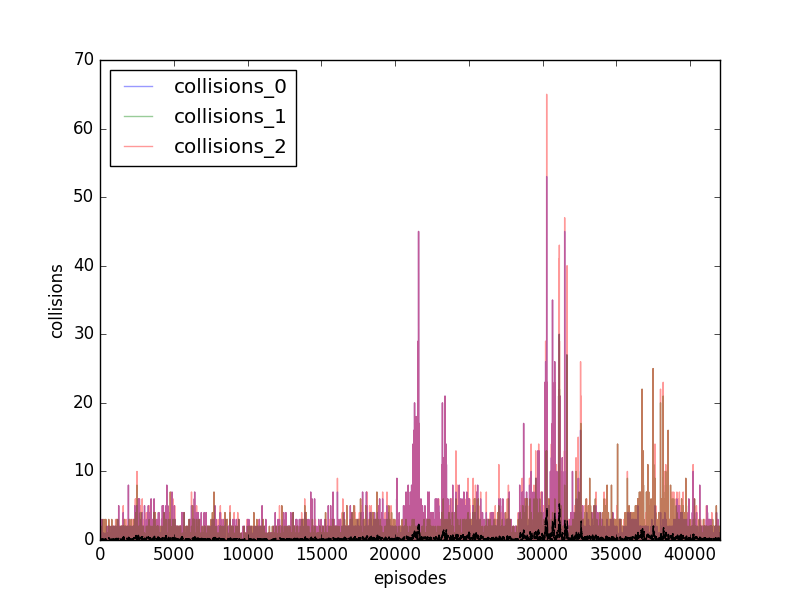
\includegraphics[trim=10 10 10 10,clip,width=\figscale\linewidth]
  {../results/maddpg_1vs2/collisions.png}
  \caption{Number of collisions per episode over training episode for MADDPG.}
  \label{fig:maddpg-1vs2}
\end{figure}
\FloatBarrier


\begin{figure}[h]
  \centering
  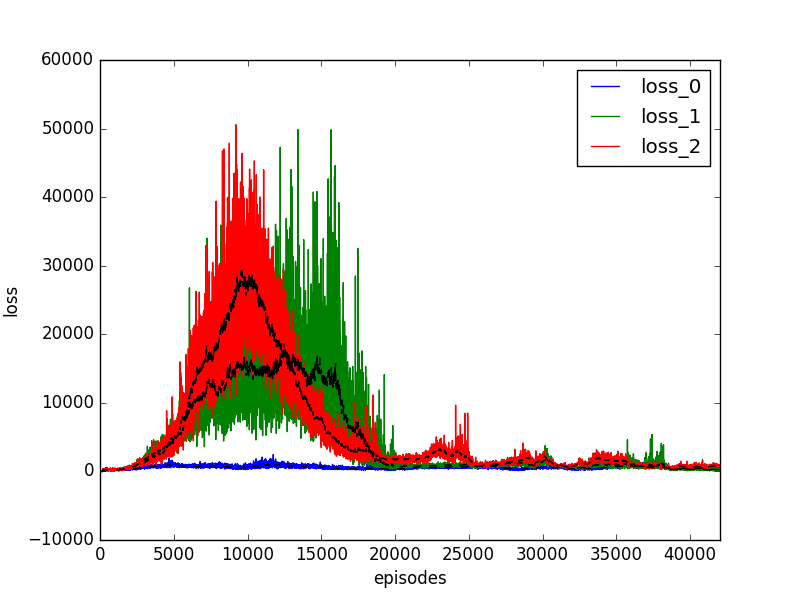
\includegraphics[trim=10 10 10 10,clip,width=\figscale\linewidth]
  {../results/maddpg_1vs2/loss.png}
  \caption{Average loss per episode over training episode for MADDPG.}
  \label{fig:maddpg-1vs2}
\end{figure}
\FloatBarrier


\subsubsection{One Agents vs. Two Adversary Results}
\label{sec:experiment:maddpg:2vs1}


\begin{figure}[h]
  \centering
  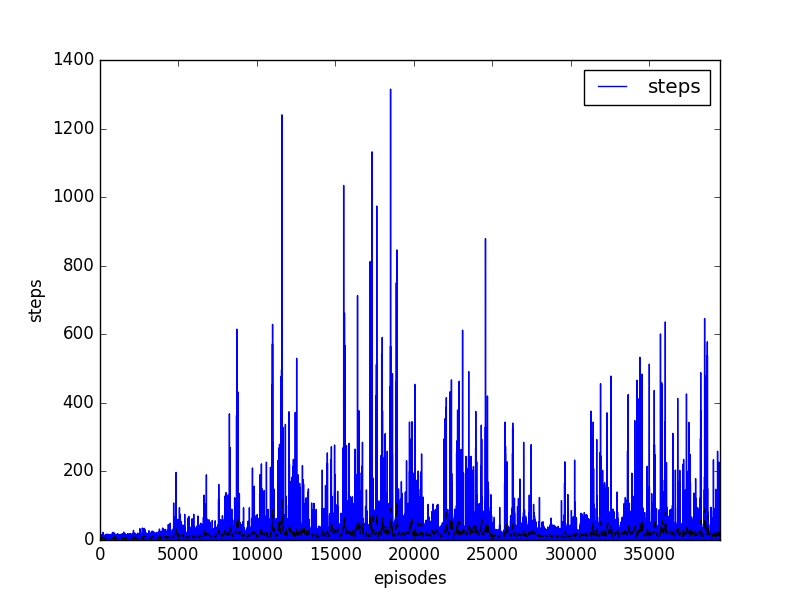
\includegraphics[trim=10 10 10 10,clip,width=\figscale\linewidth]
  {../results/maddpg_2vs1/steps.png}
  \caption{Number of steps per episode over training episode for MADDPG.}
  \label{fig:maddpg-2vs1}
\end{figure}
\FloatBarrier


\begin{figure}[h]
  \centering
  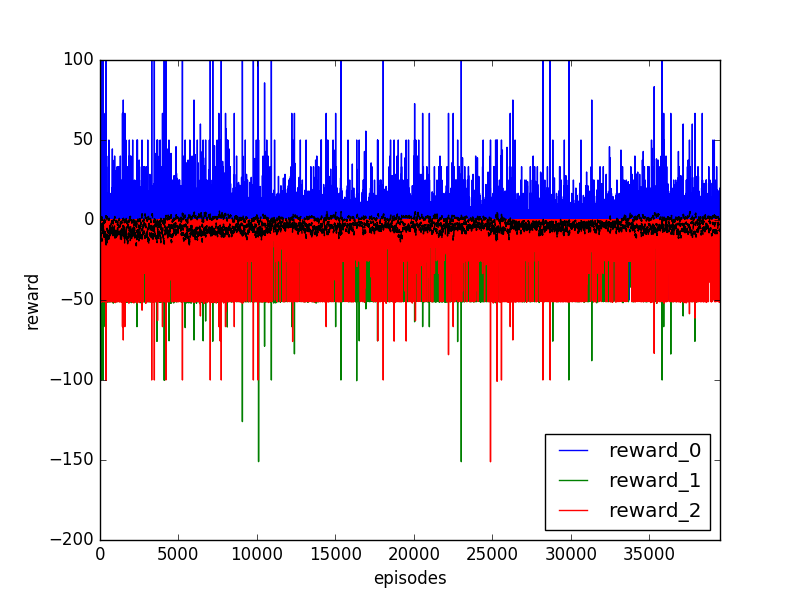
\includegraphics[trim=10 10 10 10,clip,width=\figscale\linewidth]
  {../results/maddpg_2vs1/reward.png}
  \caption{Cumulative reward per episode over training episode for MADDPG.}
  \label{fig:maddpg-2vs1}
\end{figure}
\FloatBarrier


\begin{figure}[h]
  \centering
  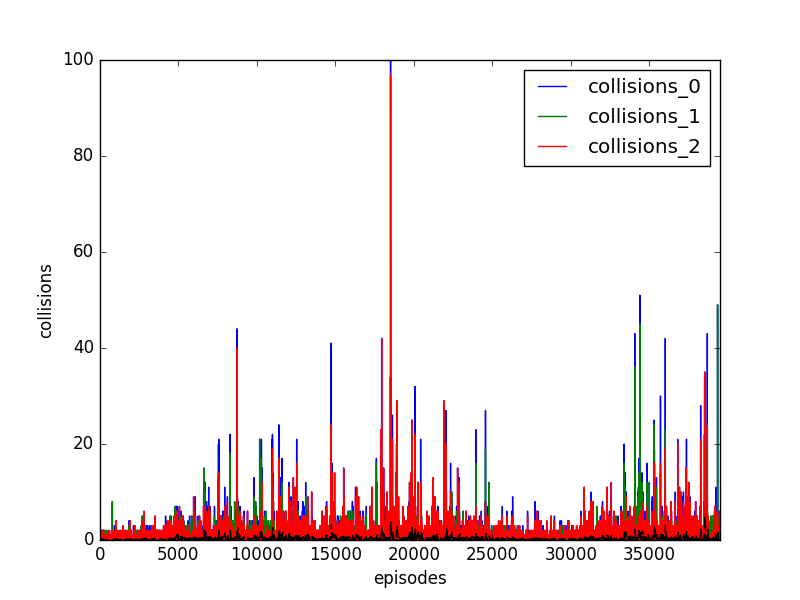
\includegraphics[trim=10 10 10 10,clip,width=\figscale\linewidth]
  {../results/maddpg_2vs1/collisions.png}
  \caption{Number of collisions per episode over training episode for MADDPG.}
  \label{fig:maddpg-2vs1}
\end{figure}
\FloatBarrier


\begin{figure}[h]
  \centering
  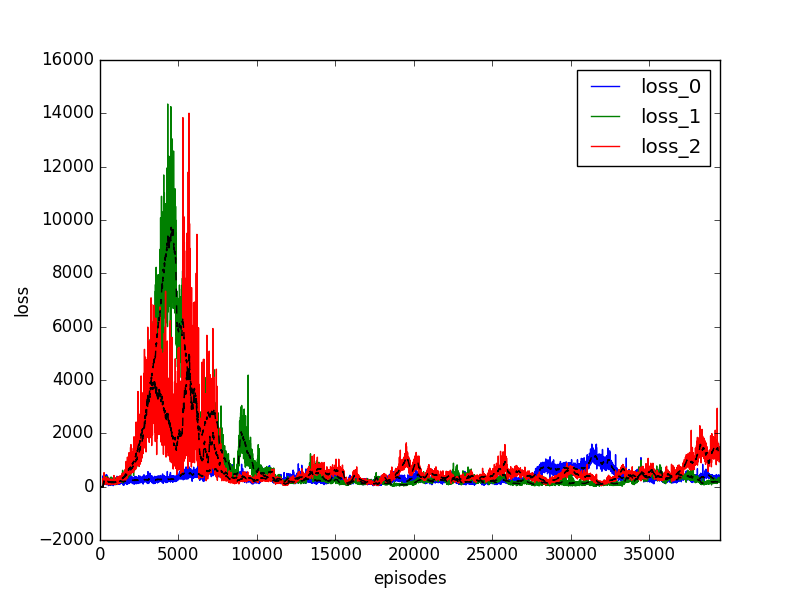
\includegraphics[trim=10 10 10 10,clip,width=\figscale\linewidth]
  {../results/maddpg_2vs1/loss.png}
  \caption{Average loss per episode over training episode for MADDPG.}
  \label{fig:maddpg-2vs1}
\end{figure}
\FloatBarrier


% !TEX root=../report.tex

\section{Future Work}
\label{sec:future}



\bibliographystyle{plain}
\bibliography{refs} %your bib file

\end{document}
